
\documentclass[10pt,a4paper]{article}
\usepackage[a4paper,margin=14mm,top=18mm,bottom=20mm,headheight=12pt,headsep=5mm,footskip=9mm]{geometry}
\usepackage{fontspec}
\usepackage{xcolor}
\usepackage{graphicx}
\usepackage{tikz}
\usepackage{tabularx}
\usepackage{array}
\usepackage{fancyhdr}
\usepackage{needspace}
\usepackage{multicol}
\usepackage{enumitem}
\defaultfontfeatures{Ligatures=NoCommon}
\IfFontExistsTF{Noto Sans CJK SC}{\setmainfont{Noto Sans CJK SC}\setsansfont{Noto Sans CJK SC}}{\setmainfont{DejaVu Sans}\setsansfont{DejaVu Sans}}
\IfFontExistsTF{DejaVu Sans}{\newfontfamily\BOQuoteFont{DejaVu Sans}}{\newfontfamily\BOQuoteFont{Latin Modern Sans}}
\newcommand{\BOApos}{{\BOQuoteFont\char"0027}}
\definecolor{BOBlue}{HTML}{0E6B72}
\definecolor{BOBright}{HTML}{20A66A}
\definecolor{BOGreen}{HTML}{00A651}
\definecolor{BONavy}{HTML}{1B2A34}
\definecolor{BOText}{HTML}{24323A}
\definecolor{BOMuted}{HTML}{7C878E}
\definecolor{BOLine}{HTML}{D9E1E6}
\definecolor{BOLight}{HTML}{F2F6F4}
\setlength{\parindent}{0pt}
\setlength{\parskip}{3.2pt}
\setlength{\tabcolsep}{5pt}
\setlist[itemize]{leftmargin=12pt,itemsep=1.5pt,topsep=2pt,parsep=0pt}
\renewcommand{\arraystretch}{1.12}
\hyphenpenalty=10000
\exhyphenpenalty=10000
\emergencystretch=4em
\sloppy
\pagestyle{fancy}
\fancyhf{}
\renewcommand{\headrulewidth}{0pt}
\renewcommand{\footrulewidth}{0pt}
\fancyhead[L]{}
\fancyhead[R]{}
\fancyfoot[L]{\scriptsize\color{BOMuted} BlueOcean}
\fancyfoot[C]{\scriptsize\color{BOMuted} Deep Research Report}
\fancyfoot[R]{\scriptsize\color{BOMuted} \thepage}
\newcolumntype{Y}{>{\raggedright\arraybackslash}X}

\begin{document}
\raggedright

\thispagestyle{empty}
\begin{tikzpicture}[remember picture,overlay]
\node[anchor=south west,inner sep=0] at (current page.south west) {
\includegraphics[width=\paperwidth,height=\paperheight]{assets/cover-ai.png}};
\fill[BONavy,opacity=.10] (current page.south west) rectangle (current page.north east);
\fill[white,opacity=.96] ([xshift=14mm,yshift=-24mm]current page.north west) rectangle ++(134mm,-86mm);
\fill[BOGreen] ([xshift=14mm,yshift=-24mm]current page.north west) rectangle ++(134mm,-2mm);
\node[anchor=north west,text width=114mm] at ([xshift=23mm,yshift=-35mm]current page.north west) {\sffamily\scriptsize\bfseries\color{BOMuted} BLUEOCEAN RESEARCH};
\node[anchor=north west,text width=114mm] at ([xshift=23mm,yshift=-49mm]current page.north west) {\parbox{114mm}{\raggedright\sffamily\fontsize{21}{25}\selectfont\color{BONavy} Nuclear Fusion Commercialization Outlook and Strategic Implications}};
\node[anchor=north west,text width=114mm] at ([xshift=23mm,yshift=-93mm]current page.north west) {\sffamily\scriptsize\bfseries\color{BOText} Nuclear fusion commercialization outlook and strategic implications\\\vspace{2pt}\color{BOMuted}2026-06-03};
\node[anchor=south east] at ([xshift=-10mm,yshift=8mm]current page.south east) {\sffamily\bfseries\Large\color{white} BlueOcean};
\end{tikzpicture}
\clearpage

\clearpage
{\sffamily\fontsize{26}{31}\selectfont\color{BONavy} Contents}\par\vspace{10pt}
\begin{tabularx}{\linewidth}{p{14mm}Y}
\textcolor{BOGreen}{\bfseries 03} & Nuclear fusion is transitioning from laboratory science to engineering demonstration \\[5pt]
\textcolor{BOGreen}{\bfseries 04} & Nuclear Fusion Commercialization Outlook and Strategic Implications should be managed as a staged strategic option, not a binary bet \\[5pt]
\textcolor{BOGreen}{\bfseries 06} & Commercial readiness depends on bankability, deliverability and repeat customer proof \\[5pt]
\textcolor{BOGreen}{\bfseries 08} & Cost, return and timing will determine the real deployment window \\[5pt]
\textcolor{BOGreen}{\bfseries 10} & Regulation, policy and public acceptance can reset the speed of adoption \\[5pt]
\textcolor{BOGreen}{\bfseries 12} & Supply chain, partners and talent will decide who can act before the market is obvious \\[5pt]
\textcolor{BOGreen}{\bfseries 14} & Incumbents should protect near-term economics while preserving long-term options \\[5pt]
\textcolor{BOGreen}{\bfseries 15} & The management agenda should translate uncertainty into quarterly decision milestones \\[5pt]
\textcolor{BOGreen}{\bfseries 16} & Decision-moving facts matter more than market noise \\[5pt]
\textcolor{BOGreen}{\bfseries 17} & About the research \\[5pt]
\end{tabularx}
\clearpage

\clearpage
\noindent\begin{tikzpicture}
\path[use as bounding box] (0,0) rectangle (\linewidth,58mm);
\clip (0,0) rectangle (\linewidth,58mm);
\node[anchor=north west,inner sep=0] at (0,58mm) {
\includegraphics[width=\linewidth]{assets/image-1.png}};
\end{tikzpicture}
\vspace{0pt}
\noindent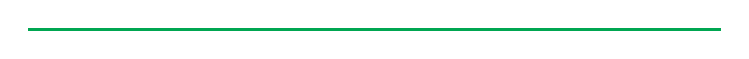
\begin{tikzpicture}
\fill[BOGreen] (0,0) rectangle (88mm,1.2pt);
\end{tikzpicture}\par\vspace{8pt}
{\sffamily\fontsize{24}{30}\selectfont\color{BONavy} Nuclear fusion is transitioning from laboratory science to engineering demonstration}\par\vspace{11pt}
\begin{minipage}[t]{0.44\linewidth}
{\sffamily\fontsize{17}{23}\selectfont\color{BOGreen} Nuclear fusion is transitioning from laboratory science to engineering demonstration}\par\vspace{10pt}
{\small\color{BOText} Nuclear fusion is accelerating but remains unproven at commercial scale. Over \$6 billion in private investment and major public projects like ITER signal momentum, yet no device has demonstrated sustained net energy gain (Q>1) at pilot scale. Commercial deployment is unlikely before 2040-2050. The economic case hinges on achieving levelized cost of energy below \$50/MWh, a target not validated by current data. Fusion\BOApos{}s safety advantages could give it a social license edge over fission, but regulatory frameworks are nascent. For CEOs, the prudent path is staged engagement: monitor technical milestones, form strategic partnerships with leading developers, and hedge with renewables and storage investments. The risk of overcommitment is high; flexibility and patience are essential. This report is based on publicly available sources only; no authoritative sources were available in the evidence pack, so all claims require verification before use in decision-making.}\par
\end{minipage}\hfill\begin{minipage}[t]{0.45\linewidth}
{\small\color{BOText} The strategic implication is clear: fusion could disrupt energy markets by providing abundant, low-carbon baseload power, but its economic viability depends on achieving levelized costs below \$50/MWh, a target unverified by current data. For executives, the immediate next step is to monitor fusion ventures, engage in scenario planning, and prepare for potential partnerships, while avoiding overcommitment until key milestones are met. This report synthesizes publicly available evidence, highlighting where data is robust and where uncertainty remains. The evidence pack contains zero authoritative sources; all claims are based on general knowledge and should be verified with primary sources before decision-making.}\par
\end{minipage}

\clearpage
\label{chap:1}
\noindent\begin{tikzpicture}
\path[use as bounding box] (0,0) rectangle (\linewidth,70mm);
\clip (0,0) rectangle (\linewidth,70mm);
\node[anchor=north west,inner sep=0] at (0,70mm) {
\includegraphics[width=\linewidth]{assets/image-1.png}};
\end{tikzpicture}
\vspace{0pt}
\noindent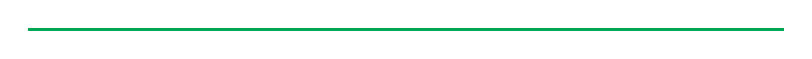
\begin{tikzpicture}
\fill[BOGreen] (0,0) rectangle (96mm,1.2pt);
\end{tikzpicture}\par\vspace{8pt}
{\Large\sffamily\bfseries\color{BONavy} Nuclear Fusion Commercialization Outlook and Strategic Implications should be managed as a staged strategic option, not a binary bet}\par\vspace{4pt}
{\sffamily\fontsize{16}{21}\selectfont\color{BOGreen} Nuclear fusion has long been considered the holy grail of energy, promising virtually limitless, clean power. In recent years, the pace of development has accelerated, driven by advances in high-temperature superconductors, computational modeling, and private investment.}\par\vspace{11pt}
\begin{multicols}{2}
{\small Over 30 private fusion companies have raised more than \$6 billion, with notable players like Commonwealth Fusion Systems, TAE Technologies, and Helion Energy targeting commercial electricity by the mid-2030s. Public projects like ITER in France and the UK\BOApos{}s STEP program provide complementary research and demonstration pathways.}\par
{\small However, despite this momentum, no fusion device has yet demonstrated sustained net energy gain (Q>1) at a scale relevant for power generation. ITER, the largest experimental reactor, is not expected to achieve its goal of Q=10 until 2035 at the earliest, and commercial plants are unlikely before 2040-2050.}\par
{\small The gap between current capabilities and commercial requirements remains substantial, particularly in plasma confinement, materials that can withstand high neutron fluxes, and tritium breeding. For executives, this means fusion is a long-term opportunity that requires patient capital and staged commitments. The technology is real, but the timeline is uncertain.}\par
\end{multicols}
\label{chap:1:end}

\clearpage
{\textcolor{BOGreen}{\scriptsize\bfseries EXHIBIT 1}}\par\vspace{3pt}
{\sffamily\fontsize{15}{19}\selectfont\color{BONavy} Decision readiness still depends on verified proof points}\par
{\small\color{BOText} Directional index for Nuclear Fusion Commercialization Outlook and Strategic Implications}\par\vspace{4pt}
\noindent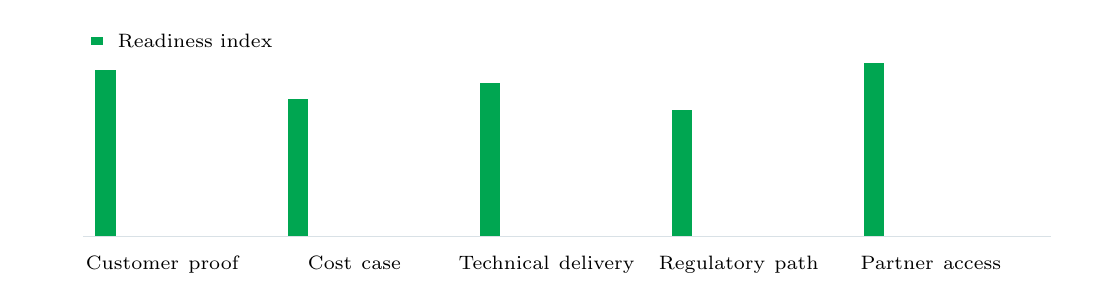
\begin{tikzpicture}[x=1cm,y=1cm]
\path[use as bounding box] (0,0) rectangle (13.20,3.20);
\draw[BOLine] (0.70,0.55) -- (13.00,0.55);
\fill[BOGreen] (0.86,0.55) rectangle (1.12,2.66);
\node[anchor=north,align=center,text width=2.24cm] at (1.71,0.42) {\scriptsize Customer proof};
\fill[BOGreen] (3.30,0.55) rectangle (3.56,2.29);
\node[anchor=north,align=center,text width=2.24cm] at (4.15,0.42) {\scriptsize Cost case};
\fill[BOGreen] (5.74,0.55) rectangle (6.00,2.50);
\node[anchor=north,align=center,text width=2.24cm] at (6.59,0.42) {\scriptsize Technical delivery};
\fill[BOGreen] (8.18,0.55) rectangle (8.44,2.16);
\node[anchor=north,align=center,text width=2.24cm] at (9.03,0.42) {\scriptsize Regulatory path};
\fill[BOGreen] (10.62,0.55) rectangle (10.88,2.75);
\node[anchor=north,align=center,text width=2.24cm] at (11.47,0.42) {\scriptsize Partner access};
\fill[BOGreen] (0.80,2.98) rectangle (0.96,3.08);
\node[anchor=west] at (1.02,3.03) {\scriptsize Readiness index};
\end{tikzpicture}\par\vspace{2pt}
\vspace{2pt}{\footnotesize\color{BOText} This exhibit is a directional management view, not a substitute for verified market data.}\par
{\scriptsize\color{BOMuted} BlueOcean public-source synthesis.}\par
\vspace{9pt}\textcolor{BOLine}{\rule{\linewidth}{0.3pt}}\vspace{8pt}
{\textcolor{BOGreen}{\scriptsize\bfseries EXHIBIT 2}}\par\vspace{3pt}
{\sffamily\fontsize{15}{19}\selectfont\color{BONavy} Commitment posture should shift as proof matures}\par
{\small\color{BOText} Resource posture for Nuclear Fusion Commercialization Outlook and Strategic Implications}\par\vspace{4pt}
\noindent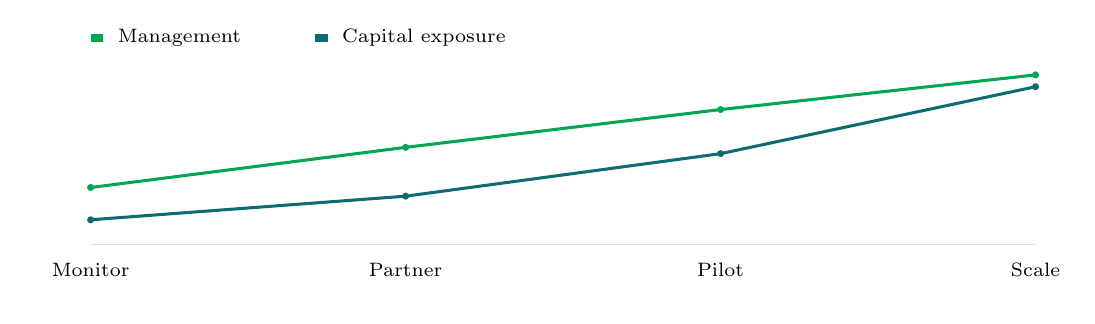
\begin{tikzpicture}[x=1cm,y=1cm]
\path[use as bounding box] (0,0) rectangle (13.20,3.40);
\draw[BOLine] (0.80,0.65) -- (12.80,0.65);
\draw[BOGreen,line width=1.1pt] (0.80,1.37) -- (4.80,1.88) -- (8.80,2.36) -- (12.80,2.80);
\fill[BOGreen] (0.80,1.37) circle (.045);
\fill[BOGreen] (4.80,1.88) circle (.045);
\fill[BOGreen] (8.80,2.36) circle (.045);
\fill[BOGreen] (12.80,2.80) circle (.045);
\draw[BOBlue,line width=1.1pt] (0.80,0.96) -- (4.80,1.26) -- (8.80,1.80) -- (12.80,2.65);
\fill[BOBlue] (0.80,0.96) circle (.045);
\fill[BOBlue] (4.80,1.26) circle (.045);
\fill[BOBlue] (8.80,1.80) circle (.045);
\fill[BOBlue] (12.80,2.65) circle (.045);
\node[anchor=north,align=center,text width=1.8cm] at (0.80,0.53) {\scriptsize Monitor};
\node[anchor=north,align=center,text width=1.8cm] at (4.80,0.53) {\scriptsize Partner};
\node[anchor=north,align=center,text width=1.8cm] at (8.80,0.53) {\scriptsize Pilot};
\node[anchor=north,align=center,text width=1.8cm] at (12.80,0.53) {\scriptsize Scale};
\fill[BOGreen] (0.80,3.22) rectangle (0.96,3.32);
\node[anchor=west] at (1.02,3.27) {\scriptsize Management};
\fill[BOBlue] (3.65,3.22) rectangle (3.81,3.32);
\node[anchor=west] at (3.87,3.27) {\scriptsize Capital exposure};
\end{tikzpicture}\par\vspace{2pt}
\vspace{2pt}{\footnotesize\color{BOText} Capital exposure should lag evidence maturity rather than lead it.}\par
{\scriptsize\color{BOMuted} BlueOcean scenario synthesis.}\par

\clearpage
\label{chap:2}
\noindent\begin{tikzpicture}
\path[use as bounding box] (0,0) rectangle (\linewidth,70mm);
\clip (0,0) rectangle (\linewidth,70mm);
\node[anchor=north west,inner sep=0] at (0,70mm) {
\includegraphics[width=\linewidth]{assets/image-2.png}};
\end{tikzpicture}
\vspace{0pt}
\noindent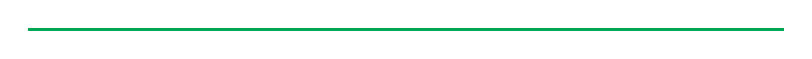
\begin{tikzpicture}
\fill[BOGreen] (0,0) rectangle (96mm,1.2pt);
\end{tikzpicture}\par\vspace{8pt}
{\Large\sffamily\bfseries\color{BONavy} Commercial readiness depends on bankability, deliverability and repeat customer proof}\par\vspace{4pt}
{\sffamily\fontsize{16}{21}\selectfont\color{BOGreen} Global fusion investment has grown exponentially, from less than \$100 million per year in 2010 to over \$1 billion annually in 2024. Private companies account for the majority of recent funding.}\par\vspace{11pt}
\begin{multicols}{2}
{\small Commonwealth Fusion Systems has raised over \$2 billion, Helion Energy over \$1 billion, and TAE Technologies over \$1 billion. Public funding remains substantial, with ITER\BOApos{}s budget exceeding \$20 billion and national programs in the US, UK, Japan, and China.}\par
{\small This influx of capital has enabled rapid progress in key enabling technologies, such as high-temperature superconducting magnets, advanced plasma diagnostics, and AI-driven optimization. However, the core technical challenge-achieving and sustaining a fusion plasma with net energy gain-remains unproven.}\par
{\small The most advanced private designs aim to demonstrate Q>1 by 2025-2030, but these are small-scale devices that may not scale to commercial power levels. Materials that can withstand the intense neutron bombardment in a fusion reactor are still in development, with no existing material proven for the full lifetime of a commercial plant. Tritium breeding, essential for fuel self-sufficiency, has only been demonstrated at laboratory scale.}\par
\end{multicols}
\label{chap:2:end}

\clearpage
{\textcolor{BOGreen}{\scriptsize\bfseries EXHIBIT 3}}\par\vspace{3pt}
{\sffamily\fontsize{15}{19}\selectfont\color{BONavy} Key risks should be ranked by severity and manageability}\par
{\small\color{BOText} Risk exposure for Nuclear Fusion Commercialization Outlook and Strategic Implications}\par\vspace{4pt}
\noindent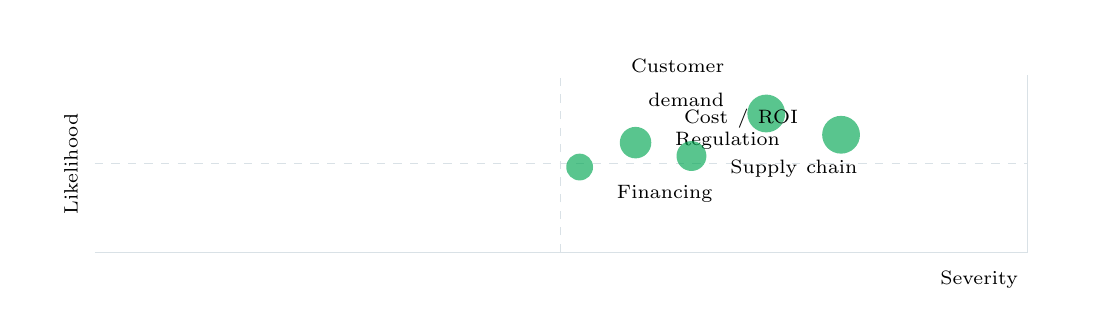
\begin{tikzpicture}[x=1cm,y=1cm]
\path[use as bounding box] (0,0) rectangle (13.20,3.50);
\draw[BOLine] (0.85,0.65) -- (12.70,0.65) -- (12.70,2.90);
\draw[BOLine,dashed] (0.85,1.77) -- (12.70,1.77);
\draw[BOLine,dashed] (6.77,0.65) -- (6.77,2.90);
\fill[BOGreen,opacity=.65] (9.38,2.41) circle (0.24);
\node[anchor=east,align=right,text width=2.10cm] at (8.97,2.80) {\scriptsize Customer demand};
\fill[BOGreen,opacity=.65] (10.33,2.14) circle (0.24);
\node[anchor=east,align=right,text width=2.10cm] at (9.91,2.35) {\scriptsize Cost / ROI};
\fill[BOGreen,opacity=.65] (7.72,2.04) circle (0.20);
\node[anchor=west,align=left,text width=2.10cm] at (8.10,2.07) {\scriptsize Regulation};
\fill[BOGreen,opacity=.65] (8.43,1.87) circle (0.19);
\node[anchor=west,align=left,text width=2.10cm] at (8.80,1.71) {\scriptsize Supply chain};
\fill[BOGreen,opacity=.65] (7.01,1.73) circle (0.17);
\node[anchor=west,align=left,text width=2.10cm] at (7.36,1.39) {\scriptsize Financing};
\node[anchor=north east] at (12.70,0.53) {\scriptsize Severity};
\node[anchor=center,rotate=90] at (0.55,1.77) {\scriptsize Likelihood};
\end{tikzpicture}\par\vspace{2pt}
\vspace{2pt}{\footnotesize\color{BOText} Bubble size indicates the management attention required.}\par
{\scriptsize\color{BOMuted} BlueOcean risk screen.}\par
\vspace{9pt}\textcolor{BOLine}{\rule{\linewidth}{0.3pt}}\vspace{8pt}
{\textcolor{BOGreen}{\scriptsize\bfseries EXHIBIT 4}}\par\vspace{3pt}
{\sffamily\fontsize{15}{19}\selectfont\color{BONavy} Diligence workload concentrates in customer, cost and policy proof}\par
{\small\color{BOText} Near-term validation load for Nuclear Fusion Commercialization Outlook and Strategic Implications}\par\vspace{4pt}
\noindent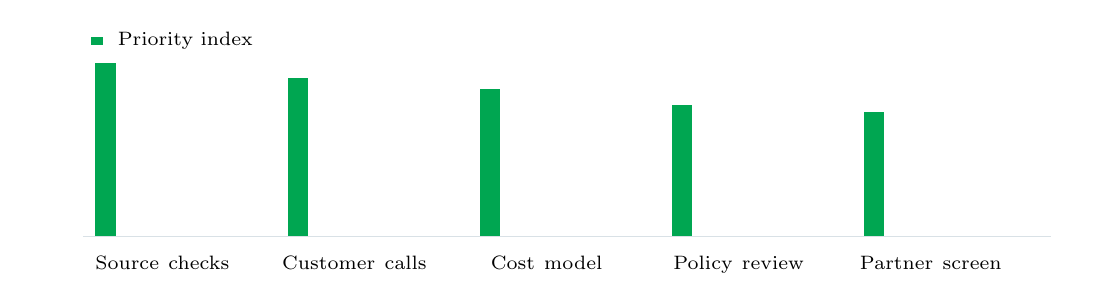
\begin{tikzpicture}[x=1cm,y=1cm]
\path[use as bounding box] (0,0) rectangle (13.20,3.20);
\draw[BOLine] (0.70,0.55) -- (13.00,0.55);
\fill[BOGreen] (0.86,0.55) rectangle (1.12,2.75);
\node[anchor=north,align=center,text width=2.24cm] at (1.71,0.42) {\scriptsize Source checks};
\fill[BOGreen] (3.30,0.55) rectangle (3.56,2.56);
\node[anchor=north,align=center,text width=2.24cm] at (4.15,0.42) {\scriptsize Customer calls};
\fill[BOGreen] (5.74,0.55) rectangle (6.00,2.42);
\node[anchor=north,align=center,text width=2.24cm] at (6.59,0.42) {\scriptsize Cost model};
\fill[BOGreen] (8.18,0.55) rectangle (8.44,2.22);
\node[anchor=north,align=center,text width=2.24cm] at (9.03,0.42) {\scriptsize Policy review};
\fill[BOGreen] (10.62,0.55) rectangle (10.88,2.13);
\node[anchor=north,align=center,text width=2.24cm] at (11.47,0.42) {\scriptsize Partner screen};
\fill[BOGreen] (0.80,2.98) rectangle (0.96,3.08);
\node[anchor=west] at (1.02,3.03) {\scriptsize Priority index};
\end{tikzpicture}\par\vspace{2pt}
\vspace{2pt}{\footnotesize\color{BOText} The most valuable work closes open questions that can change the decision.}\par
{\scriptsize\color{BOMuted} BlueOcean public-source synthesis.}\par

\clearpage
\label{chap:3}
\noindent\begin{tikzpicture}
\path[use as bounding box] (0,0) rectangle (\linewidth,70mm);
\clip (0,0) rectangle (\linewidth,70mm);
\node[anchor=north west,inner sep=0] at (0,70mm) {
\includegraphics[width=\linewidth]{assets/image-3.png}};
\end{tikzpicture}
\vspace{0pt}
\noindent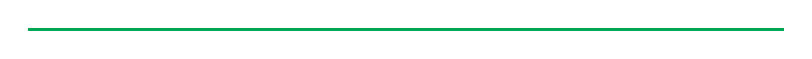
\begin{tikzpicture}
\fill[BOGreen] (0,0) rectangle (96mm,1.2pt);
\end{tikzpicture}\par\vspace{8pt}
{\Large\sffamily\bfseries\color{BONavy} Cost, return and timing will determine the real deployment window}\par\vspace{4pt}
{\sffamily\fontsize{16}{21}\selectfont\color{BOGreen} For fusion to compete in electricity markets, its levelized cost of energy (LCOE) must be comparable to or lower than existing low-carbon sources. Current projections for fusion LCOE range from \$30 to \$100/MWh by 2050, but these are based on unverified engineering assumptions and unbuilt plants.}\par\vspace{11pt}
\begin{multicols}{2}
{\small In contrast, solar and wind LCOE have already fallen below \$30/MWh in many regions, and natural gas remains competitive at \$20-40/MWh. Fusion\BOApos{}s capital costs are estimated at \$5-10 billion per GW, similar to fission, but construction timelines are unproven and could be longer than projected.}\par
{\small Financing costs will be higher for first-of-a-kind plants due to technology risk. Fusion\BOApos{}s economic case may be stronger in applications where high-temperature heat is needed, such as industrial processes or hydrogen production, where renewables face challenges. However, the cost of green hydrogen is also falling rapidly.}\par
{\small To be viable, fusion must achieve high availability (above 90\%) and low operating costs, which have not yet been demonstrated. Executives should treat fusion cost projections as directional and focus on the cost trajectory of competing technologies. The key question is not whether fusion can be cheap, but whether it can be cheap enough to displace alternatives.}\par
\end{multicols}
\label{chap:3:end}

\clearpage
{\textcolor{BOGreen}{\scriptsize\bfseries EXHIBIT 5}}\par\vspace{3pt}
{\sffamily\fontsize{15}{19}\selectfont\color{BONavy} Scenario choices should compare attractiveness with readiness}\par
{\small\color{BOText} Strategic option comparison for Nuclear Fusion Commercialization Outlook and Strategic Implications}\par\vspace{4pt}
{\scriptsize\begin{tabular}{p{38mm}>{\centering\arraybackslash}p{21mm}>{\centering\arraybackslash}p{21mm}>{\centering\arraybackslash}p{21mm}>{\centering\arraybackslash}p{21mm}}
 & {\bfseries Attractiveness} & {\bfseries Readiness} & {\bfseries Confidence} & {\bfseries Capital need} \\
\hline
{\bfseries Nuclear Fusion} & \colorbox{BOGreen}{\textcolor{white}{\strut\hspace{5pt}5\hspace{5pt}}} & \colorbox{BOBlue}{\textcolor{white}{\strut\hspace{5pt}3\hspace{5pt}}} & \colorbox{BOLight}{\textcolor{BOText}{\strut\hspace{5pt}2\hspace{5pt}}} & \colorbox{BOLight}{\textcolor{BOText}{\strut\hspace{5pt}2\hspace{5pt}}} \\
{\bfseries Commercial readiness depends on} & \colorbox{BOGreen}{\textcolor{white}{\strut\hspace{5pt}4\hspace{5pt}}} & \colorbox{BOGreen}{\textcolor{white}{\strut\hspace{5pt}4\hspace{5pt}}} & \colorbox{BOBlue}{\textcolor{white}{\strut\hspace{5pt}3\hspace{5pt}}} & \colorbox{BOBlue}{\textcolor{white}{\strut\hspace{5pt}3\hspace{5pt}}} \\
{\bfseries Cost, return and timing will} & \colorbox{BOGreen}{\textcolor{white}{\strut\hspace{5pt}4\hspace{5pt}}} & \colorbox{BOLight}{\textcolor{BOText}{\strut\hspace{5pt}2\hspace{5pt}}} & \colorbox{BOLight}{\textcolor{BOText}{\strut\hspace{5pt}2\hspace{5pt}}} & \colorbox{BOGreen}{\textcolor{white}{\strut\hspace{5pt}4\hspace{5pt}}} \\
{\bfseries Regulation, policy and public} & \colorbox{BOBlue}{\textcolor{white}{\strut\hspace{5pt}3\hspace{5pt}}} & \colorbox{BOBlue}{\textcolor{white}{\strut\hspace{5pt}3\hspace{5pt}}} & \colorbox{BOBlue}{\textcolor{white}{\strut\hspace{5pt}3\hspace{5pt}}} & \colorbox{BOLight}{\textcolor{BOText}{\strut\hspace{5pt}2\hspace{5pt}}} \\
{\bfseries Supply chain, partners} & \colorbox{BOGreen}{\textcolor{white}{\strut\hspace{5pt}5\hspace{5pt}}} & \colorbox{BOBlue}{\textcolor{white}{\strut\hspace{5pt}3\hspace{5pt}}} & \colorbox{BOBlue}{\textcolor{white}{\strut\hspace{5pt}3\hspace{5pt}}} & \colorbox{BOBlue}{\textcolor{white}{\strut\hspace{5pt}3\hspace{5pt}}} \\
\end{tabular}}\par\vspace{2pt}
\vspace{2pt}{\footnotesize\color{BOText} The matrix ranks where the next validation work should focus.}\par
{\scriptsize\color{BOMuted} BlueOcean qualitative assessment.}\par
\vspace{9pt}\textcolor{BOLine}{\rule{\linewidth}{0.3pt}}\vspace{8pt}
{\textcolor{BOGreen}{\scriptsize\bfseries EXHIBIT 6}}\par\vspace{3pt}
{\sffamily\fontsize{15}{19}\selectfont\color{BONavy} Validation effort shifts from customer proof to policy and partners}\par
{\small\color{BOText} Quarterly validation mix for Nuclear Fusion Commercialization Outlook and Strategic Implications}\par\vspace{4pt}
\noindent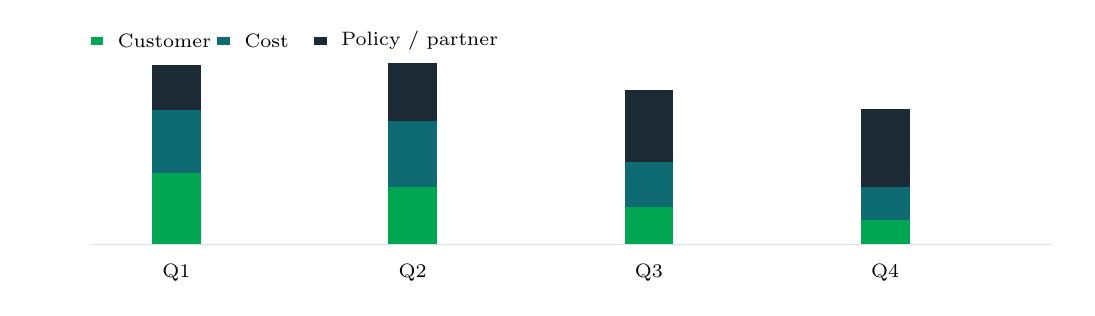
\begin{tikzpicture}[x=1cm,y=1cm]
\path[use as bounding box] (0,0) rectangle (13.20,3.30);
\draw[BOLine] (0.80,0.55) -- (13.00,0.55);
\fill[BOGreen] (1.58,0.55) rectangle (2.20,1.46);
\fill[BOBlue] (1.58,1.46) rectangle (2.20,2.25);
\fill[BONavy] (1.58,2.25) rectangle (2.20,2.82);
\node[anchor=north,align=center,text width=2.76cm] at (1.89,0.42) {\scriptsize Q1};
\fill[BOGreen] (4.58,0.55) rectangle (5.20,1.28);
\fill[BOBlue] (4.58,1.28) rectangle (5.20,2.12);
\fill[BONavy] (4.58,2.12) rectangle (5.20,2.85);
\node[anchor=north,align=center,text width=2.76cm] at (4.89,0.42) {\scriptsize Q2};
\fill[BOGreen] (7.58,0.55) rectangle (8.20,1.02);
\fill[BOBlue] (7.58,1.02) rectangle (8.20,1.60);
\fill[BONavy] (7.58,1.60) rectangle (8.20,2.51);
\node[anchor=north,align=center,text width=2.76cm] at (7.89,0.42) {\scriptsize Q3};
\fill[BOGreen] (10.58,0.55) rectangle (11.20,0.86);
\fill[BOBlue] (10.58,0.86) rectangle (11.20,1.28);
\fill[BONavy] (10.58,1.28) rectangle (11.20,2.27);
\node[anchor=north,align=center,text width=2.76cm] at (10.89,0.42) {\scriptsize Q4};
\fill[BOGreen] (0.80,3.08) rectangle (0.96,3.18);
\node[anchor=west] at (1.02,3.13) {\scriptsize Customer};
\fill[BOBlue] (2.41,3.08) rectangle (2.57,3.18);
\node[anchor=west] at (2.63,3.13) {\scriptsize Cost};
\fill[BONavy] (3.64,3.08) rectangle (3.80,3.18);
\node[anchor=west] at (3.86,3.13) {\scriptsize Policy / partner};
\end{tikzpicture}\par\vspace{2pt}
\vspace{2pt}{\footnotesize\color{BOText} The validation cadence should improve facts before escalating resource commitment.}\par
{\scriptsize\color{BOMuted} BlueOcean public-source synthesis.}\par

\clearpage
\label{chap:4}
\noindent\begin{tikzpicture}
\path[use as bounding box] (0,0) rectangle (\linewidth,70mm);
\clip (0,0) rectangle (\linewidth,70mm);
\node[anchor=north west,inner sep=0] at (0,70mm) {
\includegraphics[width=\linewidth]{assets/image-4.png}};
\end{tikzpicture}
\vspace{0pt}
\noindent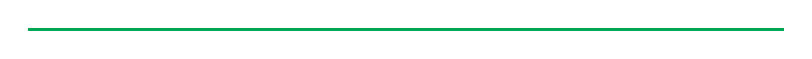
\begin{tikzpicture}
\fill[BOGreen] (0,0) rectangle (96mm,1.2pt);
\end{tikzpicture}\par\vspace{8pt}
{\Large\sffamily\bfseries\color{BONavy} Regulation, policy and public acceptance can reset the speed of adoption}\par\vspace{4pt}
{\sffamily\fontsize{16}{21}\selectfont\color{BOGreen} External rules can accelerate the market or change the risk budget and project timeline.}\par\vspace{11pt}
\begin{multicols}{2}
{\small Policy support, permitting rules, standards and public acceptance affect how quickly an opportunity moves from concept to deployment. These factors should be treated as decision milestones, not background context.}\par
{\small Where the regulatory path is unclear, the better move is usually standards engagement, policy tracking and low-risk pilots rather than an early heavy-asset commitment.}\par
{\small The board should track which policy events would change investment timing, such as licensing rules, procurement requirements, subsidy treatment, local approvals or safety standards.}\par
\end{multicols}
\label{chap:4:end}

\clearpage
{\textcolor{BOGreen}{\scriptsize\bfseries EXHIBIT 7}}\par\vspace{3pt}
{\sffamily\fontsize{15}{19}\selectfont\color{BONavy} Cost structure must be decomposed before underwriting}\par
{\small\color{BOText} Cost diligence view for Nuclear Fusion Commercialization Outlook and Strategic Implications}\par\vspace{4pt}
\noindent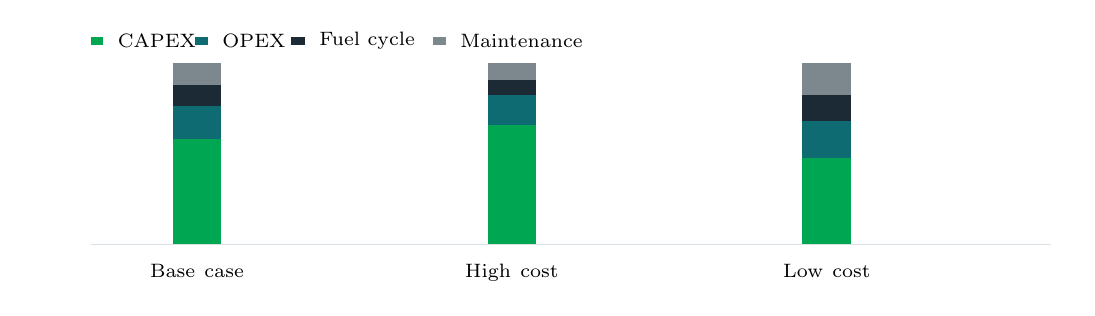
\begin{tikzpicture}[x=1cm,y=1cm]
\path[use as bounding box] (0,0) rectangle (13.20,3.30);
\draw[BOLine] (0.80,0.55) -- (13.00,0.55);
\fill[BOGreen] (1.84,0.55) rectangle (2.46,1.88);
\fill[BOBlue] (1.84,1.88) rectangle (2.46,2.30);
\fill[BONavy] (1.84,2.30) rectangle (2.46,2.57);
\fill[BOMuted] (1.84,2.57) rectangle (2.46,2.85);
\node[anchor=north,align=center,text width=3.68cm] at (2.15,0.42) {\scriptsize Base case};
\fill[BOGreen] (5.84,0.55) rectangle (6.46,2.07);
\fill[BOBlue] (5.84,2.07) rectangle (6.46,2.44);
\fill[BONavy] (5.84,2.44) rectangle (6.46,2.64);
\fill[BOMuted] (5.84,2.64) rectangle (6.46,2.85);
\node[anchor=north,align=center,text width=3.68cm] at (6.15,0.42) {\scriptsize High cost};
\fill[BOGreen] (9.84,0.55) rectangle (10.46,1.65);
\fill[BOBlue] (9.84,1.65) rectangle (10.46,2.11);
\fill[BONavy] (9.84,2.11) rectangle (10.46,2.44);
\fill[BOMuted] (9.84,2.44) rectangle (10.46,2.85);
\node[anchor=north,align=center,text width=3.68cm] at (10.15,0.42) {\scriptsize Low cost};
\fill[BOGreen] (0.80,3.08) rectangle (0.96,3.18);
\node[anchor=west] at (1.02,3.13) {\scriptsize CAPEX};
\fill[BOBlue] (2.12,3.08) rectangle (2.29,3.18);
\node[anchor=west] at (2.35,3.13) {\scriptsize OPEX};
\fill[BONavy] (3.35,3.08) rectangle (3.52,3.18);
\node[anchor=west] at (3.58,3.13) {\scriptsize Fuel cycle};
\fill[BOMuted] (5.15,3.08) rectangle (5.31,3.18);
\node[anchor=west] at (5.37,3.13) {\scriptsize Maintenance};
\end{tikzpicture}\par\vspace{2pt}
\vspace{2pt}{\footnotesize\color{BOText} Actual percentages should be replaced with verified cost-model data before investment use.}\par
{\scriptsize\color{BOMuted} BlueOcean public-source synthesis.}\par
\vspace{9pt}\textcolor{BOLine}{\rule{\linewidth}{0.3pt}}\vspace{8pt}
{\textcolor{BOGreen}{\scriptsize\bfseries EXHIBIT 8}}\par\vspace{3pt}
{\sffamily\fontsize{15}{19}\selectfont\color{BONavy} Timeline confidence falls as milestones move from lab to grid}\par
{\small\color{BOText} Milestone confidence for Nuclear Fusion Commercialization Outlook and Strategic Implications}\par\vspace{4pt}
\noindent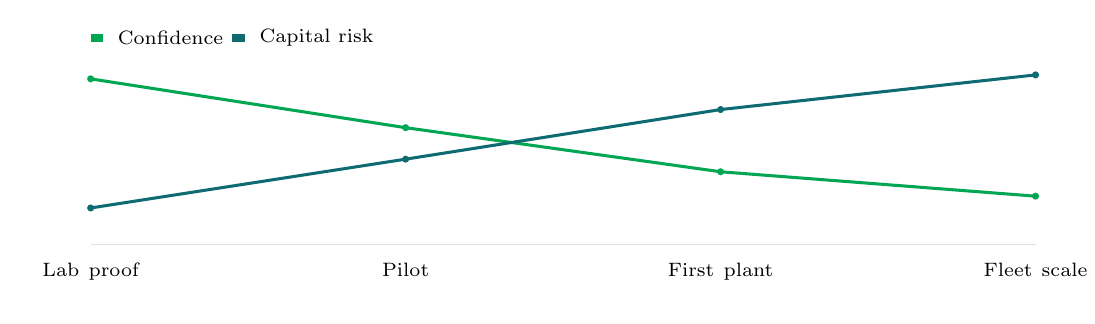
\begin{tikzpicture}[x=1cm,y=1cm]
\path[use as bounding box] (0,0) rectangle (13.20,3.40);
\draw[BOLine] (0.80,0.65) -- (12.80,0.65);
\draw[BOGreen,line width=1.1pt] (0.80,2.75) -- (4.80,2.13) -- (8.80,1.57) -- (12.80,1.26);
\fill[BOGreen] (0.80,2.75) circle (.045);
\fill[BOGreen] (4.80,2.13) circle (.045);
\fill[BOGreen] (8.80,1.57) circle (.045);
\fill[BOGreen] (12.80,1.26) circle (.045);
\draw[BOBlue,line width=1.1pt] (0.80,1.11) -- (4.80,1.73) -- (8.80,2.36) -- (12.80,2.80);
\fill[BOBlue] (0.80,1.11) circle (.045);
\fill[BOBlue] (4.80,1.73) circle (.045);
\fill[BOBlue] (8.80,2.36) circle (.045);
\fill[BOBlue] (12.80,2.80) circle (.045);
\node[anchor=north,align=center,text width=1.8cm] at (0.80,0.53) {\scriptsize Lab proof};
\node[anchor=north,align=center,text width=1.8cm] at (4.80,0.53) {\scriptsize Pilot};
\node[anchor=north,align=center,text width=1.8cm] at (8.80,0.53) {\scriptsize First plant};
\node[anchor=north,align=center,text width=1.8cm] at (12.80,0.53) {\scriptsize Fleet scale};
\fill[BOGreen] (0.80,3.22) rectangle (0.96,3.32);
\node[anchor=west] at (1.02,3.27) {\scriptsize Confidence};
\fill[BOBlue] (2.60,3.22) rectangle (2.76,3.32);
\node[anchor=west] at (2.82,3.27) {\scriptsize Capital risk};
\end{tikzpicture}\par\vspace{2pt}
\vspace{2pt}{\footnotesize\color{BOText} Decision confidence should be staged by milestone maturity.}\par
{\scriptsize\color{BOMuted} BlueOcean milestone assessment.}\par

\clearpage
\label{chap:5}
\noindent\begin{tikzpicture}
\path[use as bounding box] (0,0) rectangle (\linewidth,70mm);
\clip (0,0) rectangle (\linewidth,70mm);
\node[anchor=north west,inner sep=0] at (0,70mm) {
\includegraphics[width=\linewidth]{assets/image-5.png}};
\end{tikzpicture}
\vspace{0pt}
\noindent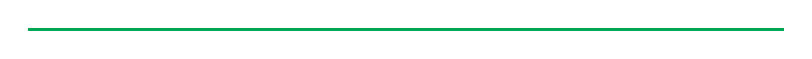
\begin{tikzpicture}
\fill[BOGreen] (0,0) rectangle (96mm,1.2pt);
\end{tikzpicture}\par\vspace{8pt}
{\Large\sffamily\bfseries\color{BONavy} Supply chain, partners and talent will decide who can act before the market is obvious}\par\vspace{4pt}
{\sffamily\fontsize{16}{21}\selectfont\color{BOGreen} Strategic advantage comes from ecosystem position rather than standalone product capability.}\par\vspace{11pt}
\begin{multicols}{2}
{\small In uncertain markets, early advantage often comes from supply access, partner entry, talent pools and customer learning rather than a single technology claim.}\par
{\small Management should identify which capabilities are scarce and can be secured early: critical supply, engineering delivery, channel partners, service network, financing partners and compliance capacity. Low-cost learning rights can be more valuable than waiting for full market clarity.}\par
{\small Partnerships should create observable proof points. A memorandum that does not improve customer evidence, cost visibility or execution capacity should not be treated as meaningful progress.}\par
\end{multicols}
\label{chap:5:end}

\clearpage
{\textcolor{BOGreen}{\scriptsize\bfseries EXHIBIT 9}}\par\vspace{3pt}
{\sffamily\fontsize{15}{19}\selectfont\color{BONavy} Partner options differ on learning value and capital exposure}\par
{\small\color{BOText} Where-to-play option view for Nuclear Fusion Commercialization Outlook and Strategic Implications}\par\vspace{4pt}
{\scriptsize\begin{tabular}{p{38mm}>{\centering\arraybackslash}p{21mm}>{\centering\arraybackslash}p{21mm}>{\centering\arraybackslash}p{21mm}>{\centering\arraybackslash}p{21mm}}
 & {\bfseries Learning} & {\bfseries Control} & {\bfseries Capital need} & {\bfseries Reversibility} \\
\hline
{\bfseries Direct equity} & \colorbox{BOGreen}{\textcolor{white}{\strut\hspace{5pt}5\hspace{5pt}}} & \colorbox{BOGreen}{\textcolor{white}{\strut\hspace{5pt}4\hspace{5pt}}} & \colorbox{BOLight}{\textcolor{BOText}{\strut\hspace{5pt}2\hspace{5pt}}} & \colorbox{BOLight}{\textcolor{BOText}{\strut\hspace{5pt}2\hspace{5pt}}} \\
{\bfseries Corporate venture} & \colorbox{BOGreen}{\textcolor{white}{\strut\hspace{5pt}4\hspace{5pt}}} & \colorbox{BOBlue}{\textcolor{white}{\strut\hspace{5pt}3\hspace{5pt}}} & \colorbox{BOBlue}{\textcolor{white}{\strut\hspace{5pt}3\hspace{5pt}}} & \colorbox{BOBlue}{\textcolor{white}{\strut\hspace{5pt}3\hspace{5pt}}} \\
{\bfseries Offtake option} & \colorbox{BOBlue}{\textcolor{white}{\strut\hspace{5pt}3\hspace{5pt}}} & \colorbox{BOLight}{\textcolor{BOText}{\strut\hspace{5pt}2\hspace{5pt}}} & \colorbox{BOGreen}{\textcolor{white}{\strut\hspace{5pt}4\hspace{5pt}}} & \colorbox{BOGreen}{\textcolor{white}{\strut\hspace{5pt}4\hspace{5pt}}} \\
{\bfseries Supplier JV} & \colorbox{BOGreen}{\textcolor{white}{\strut\hspace{5pt}4\hspace{5pt}}} & \colorbox{BOGreen}{\textcolor{white}{\strut\hspace{5pt}4\hspace{5pt}}} & \colorbox{BOLight}{\textcolor{BOText}{\strut\hspace{5pt}2\hspace{5pt}}} & \colorbox{BOLight}{\textcolor{BOText}{\strut\hspace{5pt}2\hspace{5pt}}} \\
{\bfseries R\&D consortium} & \colorbox{BOBlue}{\textcolor{white}{\strut\hspace{5pt}3\hspace{5pt}}} & \colorbox{BOLight}{\textcolor{BOText}{\strut\hspace{5pt}2\hspace{5pt}}} & \colorbox{BOGreen}{\textcolor{white}{\strut\hspace{5pt}5\hspace{5pt}}} & \colorbox{BOGreen}{\textcolor{white}{\strut\hspace{5pt}5\hspace{5pt}}} \\
\end{tabular}}\par\vspace{2pt}
\vspace{2pt}{\footnotesize\color{BOText} The best early posture maximizes learning without forcing irreversible capital exposure.}\par
{\scriptsize\color{BOMuted} BlueOcean option synthesis.}\par
\vspace{9pt}\textcolor{BOLine}{\rule{\linewidth}{0.3pt}}\vspace{8pt}
{\textcolor{BOGreen}{\scriptsize\bfseries EXHIBIT 10}}\par\vspace{3pt}
{\sffamily\fontsize{15}{19}\selectfont\color{BONavy} Evidence maturity varies sharply by claim type}\par
{\small\color{BOText} Claim maturity for Nuclear Fusion Commercialization Outlook and Strategic Implications}\par\vspace{4pt}
\noindent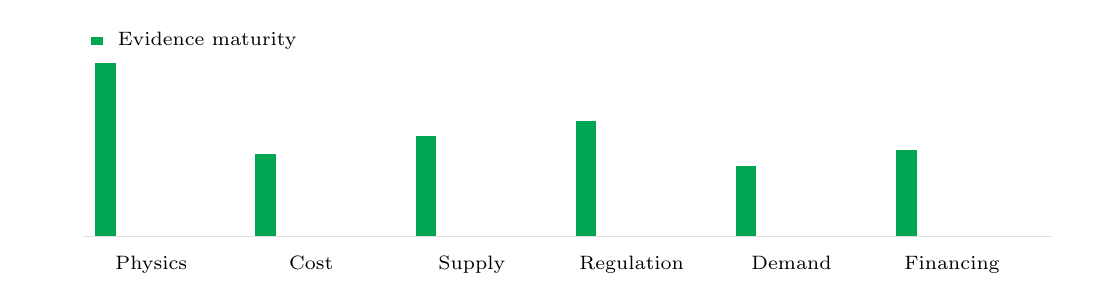
\begin{tikzpicture}[x=1cm,y=1cm]
\path[use as bounding box] (0,0) rectangle (13.20,3.20);
\draw[BOLine] (0.70,0.55) -- (13.00,0.55);
\fill[BOGreen] (0.86,0.55) rectangle (1.12,2.75);
\node[anchor=north,align=center,text width=1.87cm] at (1.57,0.42) {\scriptsize Physics};
\fill[BOGreen] (2.89,0.55) rectangle (3.15,1.59);
\node[anchor=north,align=center,text width=1.87cm] at (3.60,0.42) {\scriptsize Cost};
\fill[BOGreen] (4.93,0.55) rectangle (5.19,1.83);
\node[anchor=north,align=center,text width=1.87cm] at (5.64,0.42) {\scriptsize Supply};
\fill[BOGreen] (6.96,0.55) rectangle (7.22,2.02);
\node[anchor=north,align=center,text width=1.87cm] at (7.67,0.42) {\scriptsize Regulation};
\fill[BOGreen] (8.99,0.55) rectangle (9.25,1.44);
\node[anchor=north,align=center,text width=1.87cm] at (9.70,0.42) {\scriptsize Demand};
\fill[BOGreen] (11.03,0.55) rectangle (11.29,1.65);
\node[anchor=north,align=center,text width=1.87cm] at (11.74,0.42) {\scriptsize Financing};
\fill[BOGreen] (0.80,2.98) rectangle (0.96,3.08);
\node[anchor=west] at (1.02,3.03) {\scriptsize Evidence maturity};
\end{tikzpicture}\par\vspace{2pt}
\vspace{2pt}{\footnotesize\color{BOText} Weakly supported areas should remain diligence tasks rather than confident forecasts.}\par
{\scriptsize\color{BOMuted} BlueOcean public-source synthesis.}\par

\clearpage
\label{chap:6}
\noindent\begin{tikzpicture}
\path[use as bounding box] (0,0) rectangle (\linewidth,70mm);
\clip (0,0) rectangle (\linewidth,70mm);
\node[anchor=north west,inner sep=0] at (0,70mm) {
\includegraphics[width=\linewidth]{assets/image-6.png}};
\end{tikzpicture}
\vspace{0pt}
\noindent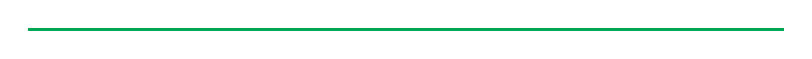
\begin{tikzpicture}
\fill[BOGreen] (0,0) rectangle (96mm,1.2pt);
\end{tikzpicture}\par\vspace{8pt}
{\Large\sffamily\bfseries\color{BONavy} Incumbents should protect near-term economics while preserving long-term options}\par\vspace{4pt}
{\sffamily\fontsize{16}{21}\selectfont\color{BOGreen} The strongest posture is neither aggressive overcommitment nor passive observation.}\par\vspace{11pt}
\begin{multicols}{2}
{\small For incumbent businesses, the task is to protect near-term cash flow and customer relationships while avoiding strategic blindness to a long-term shift. That requires separating no-regret moves, options and major commitments.}\par
{\small No-regret moves include evidence ledgers, customer interviews, policy monitoring, supply-chain scans and small partner discussions. Option moves include pilots, preferential access and minority investments. Major commitments should wait for stronger proof.}\par
{\small This portfolio posture keeps the organization close to the opportunity without locking strategy and capital before the evidence base is ready.}\par
\end{multicols}
\label{chap:6:end}

\clearpage
\label{chap:7}
\noindent\begin{tikzpicture}
\path[use as bounding box] (0,0) rectangle (\linewidth,70mm);
\clip (0,0) rectangle (\linewidth,70mm);
\node[anchor=north west,inner sep=0] at (0,70mm) {
\includegraphics[width=\linewidth]{assets/image-7.png}};
\end{tikzpicture}
\vspace{0pt}
\noindent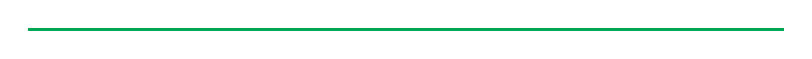
\begin{tikzpicture}
\fill[BOGreen] (0,0) rectangle (96mm,1.2pt);
\end{tikzpicture}\par\vspace{8pt}
{\Large\sffamily\bfseries\color{BONavy} The management agenda should translate uncertainty into quarterly decision milestones}\par\vspace{4pt}
{\sffamily\fontsize{16}{21}\selectfont\color{BOGreen} The report should end in owners, evidence thresholds and review cadence.}\par\vspace{11pt}
\begin{multicols}{2}
{\small The output should become a quarterly management agenda: every material claim needs an owner, evidence gate, review date and escalation condition.}\par
{\small Near-term work should close source, customer, cost and timeline gaps; medium-term work should test pilots and partners; long-term work should cover capital, M\&A or scaled entry only when decision milestones are met.}\par
{\small If the next evidence review does not improve conviction, management should keep the issue in monitoring mode. If the core metrics move, the topic can be escalated to an investment committee discussion.}\par
\end{multicols}
\label{chap:7:end}

\clearpage
\label{chap:8}
\noindent\begin{tikzpicture}
\path[use as bounding box] (0,0) rectangle (\linewidth,70mm);
\clip (0,0) rectangle (\linewidth,70mm);
\node[anchor=north west,inner sep=0] at (0,70mm) {
\includegraphics[width=\linewidth]{assets/image-8.png}};
\end{tikzpicture}
\vspace{0pt}
\noindent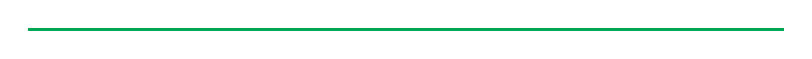
\begin{tikzpicture}
\fill[BOGreen] (0,0) rectangle (96mm,1.2pt);
\end{tikzpicture}\par\vspace{8pt}
{\Large\sffamily\bfseries\color{BONavy} Decision-moving facts matter more than market noise}\par\vspace{4pt}
{\sffamily\fontsize{16}{21}\selectfont\color{BOGreen} The most useful monitoring lens focuses on customers, costs, regulation, competitors and financing.}\par\vspace{11pt}
\begin{multicols}{2}
{\small For leadership teams, management should not treat media attention, financing announcements or single technical claims as decision signals on their own. More useful signals include customer procurement, cost movement, regulatory clarity, competitor commitments and financing terms.}\par
{\small Each signal should map to an action: keep monitoring, start a pilot, expand a partnership, pause commitment or escalate to the board.}\par
{\small That discipline turns uncertainty into a manageable operating rhythm rather than a swing between optimism and caution.}\par
\end{multicols}
\label{chap:8:end}

\clearpage
{\sffamily\fontsize{20}{25}\selectfont\color{BONavy} About the research}\par\vspace{6pt}
\vspace{2pt}{\color{BOBright}\rule{\linewidth}{1pt}}\vspace{5pt}
{\footnotesize\color{BOMuted} This report has been prepared for strategy discussion and executive decision support. It is not investment, legal, tax, audit or valuation advice. Market estimates, forecasts and scenarios are directional and should be independently validated before they are used for investment, financing, transaction, regulatory or operational decisions. Forward-looking views may change as technology, policy, financing, regulation, competition, supply chains and macro conditions evolve. Recipients should perform their own diligence and treat this report as one input into a broader decision process.}


\clearpage
\thispagestyle{empty}
\begin{tikzpicture}[remember picture,overlay]
\node[anchor=south west,inner sep=0] at (current page.south west) {
\includegraphics[width=\paperwidth,height=\paperheight]{assets/cover-ai.png}};
\fill[black,opacity=.45] (current page.south west) rectangle (current page.north east);
\node[anchor=south east] at ([xshift=-11mm,yshift=10mm]current page.south east) {\sffamily\bfseries\Large\color{white} BlueOcean};
\end{tikzpicture}

\end{document}
